\section{Вступление}
Экосистема Asure состоит из сети Asure, блокчейна Asure, платформы Asure и других сторонних приложений. 

\begin{figure}[H]
    \centering
    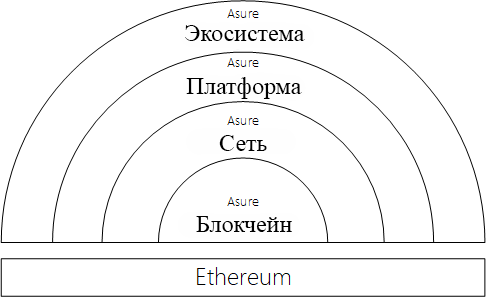
\includegraphics[width=4.0in]{img/ecosystem.png}
    \caption{Экосистема Asure}
    \label{fig:asure_ecosystem}
\end{figure}

Сеть Asure это масштабируемая блокчейн сеть для децентрализованных систем социального обеспечения. Asure закладывает основу для доступа 10 миллиардов людей к системам социального обеспечения и обеспечивает огромное социальное воздействие там, где это больше всего необходимо. \cite{worldometers} 

Являясь технологической базой, которая обеспечивает оптимальную производительность в отношении пропускной способности транзакций при сохранении децентрализованного характера сети, она гарантирует требуемый уровень прозрачности и экономической эффективности в системе. Сеть реализована в виде множества боковых цепей Plasma, которые связаны с блокчейном Asure, а также с блокчейном Ethereum или любым другим EVM-совместимым блокчейном. Каждый сайдчейн управляется несколькими независимыми провайдерами узлов, которым необходимо иметь долю токенов ASR для достижения консенсуса между ними и следовательно, внутри сети. Имея долю токенов ASR, провайдеры узлов могут зарабатывать дополнительные токены, предоставляя свою вычислительную мощность. Для каждой системы социального обеспечения в сети Asure будет сайдчейн.

Блокчейн Asure содержит рутчейн Asure и связанные сайдчейны. Рутчейн предлагает преимущества как в области безопасности, так и в области межцепной связи. Все работающие узлы блокчейна Asure представляют Asure Network. Платформа Asure соединяет бэкэнд-инфраструктуру с приложениями, которые могут использоваться конечными пользователями или программными интерфейсами для разработчиков, чтобы создавать приложения поверх платформы Asure. 


\subsection{Системы социального обеспечения}
Социальное обеспечение это система страхования, в которой застрахованные риски (такие как болезнь, материнство, потребность в длительном уходе, несчастные случаи на работе, связанные с работой заболевания, безработица, снижение трудоспособности, старость и смерть) покрываются совместно всеми застрахованными лицами. Системы социального обеспечения абсорбируют многие жизненные риски, предотвращают чрезвычайные трудности и таким образом это создет социальный баланс. 

Люди, которые не имеют доступа к системам социального обеспечения, рискуют стать нищими, если их постигнет судьба, такая как болезнь, неурожайность или инвалидность. Тогда им, возможно придется обналичить сбережения, продать скот и другие средства производства и отправить своих детей на работу вместо школы, чтобы найти финансы на ежедневные расходы. \cite{erd}

Люди, которые пользуются базовым социальным обеспечением, более склонны вкладывать средства в образование и физический капитал, что сопряжено с дополнительными рисками, но и  перспективой улучшения доходов. Эмпирические исследования показывают, что существование систем социального обеспечения, особенно в неформальном секторе, усиливает склонность к инвестициям и таким образом способствует экономическому росту именно там, где это наилучшим образом способствует сокращению бедности. \cite{hcms}

Существует широкий спектр систем социального обеспечения и все они различаются по своему конкретному применению. Для целей данного документа мы определяем функциональность наиболее распространенных систем социального обеспечения следующим образом:

\subsubsection*{Пенсия}
Пенсионная система состоит из ряда вкладчиков и пенсионеров. Участники системы платят ежемесячные страховые взносы, которые перераспределяются на нынешних пенсионеров. Взамен вкладчики имеют право на получение своей пенсии по истечении определенного периода времени, исходя из времени и суммы уплаченных взносов. В некоторых системах страховые взносы выплачиваются компанией от имени участника, что означает значительное сокращение необходимых транзакций.
Выплаты пенсий обычно происходят в установленный день, и все пенсионеры получают выплаты одновременно. Это делает его идеальным вариантом использования для транзакций массовых выплат.

\subsubsection*{Здравоохранение}
Стороны в сфере здравоохранения разнообразны, есть застрахованные люди которые платят премию, есть врачи, больницы, аптеки и другие поставщики услуг, которые выставляют счета. Они могут быть компенсированы системой или через застрахованного, который отправляет счета в систему и получает возмещенные расходы. Здесь существуют различные возможности реализации обработки партиями, застрахованный может представить накопленные счета в конце года, или врачи, больницы, аптеки и другие поставщики услуг также могут представлять свои коллективные счета партиями.

\subsubsection*{Безработица}
Страхование по безработице это защита от потери работы. Участники имеющие работу, оплачивают премию, в случае потери работы у участников есть время, чтобы найти работу снова.

\subsubsection*{Страхование социального обеспечения}

Страхование социального обеспечения, это страхование по долгосрочному уходу или страхование по уходу являющееся обязательным страхованием для покрытия риска зависимого от долгосрочного ухода. Пособия по социальному страхованию предоставляются на основе "уровней потребности в долгосрочном уходе". В случае профессиональной, амбулаторной или (частично) стационарной помощи, расходы покрываются до определенной максимальной суммы (включая средства по уходу, меры по улучшению жизненной среды, а также пособия по добровольному уходу). Поэтому обязательное социальное страхование не является полной страховкой. Чтобы получить полное покрытие, необходимо оформить частную дополнительную страховку по уходу. В случае необходимости застрахованное лицо имеет право на помощь по уходу в качестве дополнительного социального пособия, ориентированного на потребности.

\subsubsection*{Поддержка детей и молодежи}
В Германии, поддержка детей и молодежи охватывает все услуги и задачи государственных и независимых учреждений, работающих на благо молодежи и их семей. Благополучие детей и молодежи не является главной опорой социального страхования, но в основном обеспечивается независимыми учреждениями, которые тесно сотрудничают с властями. Он в основном финансируется за счет денег налогоплательщиков. 

\subsubsection*{Страхование от инвалидности / Страхование от несчастных случаев}
Целью обязательного страхования от несчастных случаев является предотвращение несчастных случаев на производстве, профессиональных заболеваний и связанных с работой рисков для здоровья, а также восстановление здоровья и профессиональной деятельности застрахованных лиц "всеми соответствующими средствами" в случае наступления этих страховых случаев.

\subsection{Блокчейн}
Блокчейн - это децентрализованная база данных, которая содержит постоянно растущий список записей транзакций. База данных расширена хронологически линейно, подобно цепочке, в которую постоянно добавляются новые элементы внизу (отсюда и термин "блокчейн"). Если блок завершен, создается следующий. Каждый блок содержит контрольную сумму предыдущего блока. Сатоши Накамото разработал Биткойн в 2009 году являясь одной из первых реализаций блокчейна, которая демонстрирует потенциал технологии для финансовых транзакций. \cite{bitcoin}

Прорывной потенциал блокчейна становится все более очевидным. После изобретения блокчейна Ethereum и виртуальной машины Ethereum (EVM) миру были предоставлены инструменты, необходимые для создания работающих децентрализованных автономных организаций (DAO). В такой системе несколько органов управления контролируют разные компоненты, и ни один из них не является полностью доверенным для всех остальных. \cite{cammarden} Технология блокчейн идеально подходит для автономного и децентрализованного социального обеспечения.